\section{Demonstration Cases}

\subsection{9.1 Benchmark Objective}

This section reports an operational demonstration of the PCS workflow using the first benchmark dataset assembled for the interval 2000--2024. The objective is limited: the benchmark tests whether the projection construction produces internally consistent annual trajectories from available public observations. No predictive claim is made, and the demonstration should not be interpreted as validation of forecasting skill.

The present benchmark includes two available projections, \(L_T\) and \(L_C\), derived from NASA GISTEMP temperature anomaly and NOAA Mauna Loa CO2, respectively. The structural projection \(L_S\) and informational projection \(L_I\) remain unavailable in this run and are retained as missing values rather than inferred.

\subsection{9.2 Data Sources}

The processed benchmark dataset contains annual values for `Year`, `Temperature`, `CO2`, `SeaLevel`, and `NDVI`. Temperature is preserved in degrees C anomaly relative to the NASA GISTEMP baseline, and CO2 is preserved in ppm. Sea level and NDVI are retained as `NaN` for all benchmark years because the corresponding sources require authenticated or manual Earthdata processing in the current run.

Unavailable projections remain missing rather than inferred. This convention preserves the distinction between an operational demonstration based on available projections and a complete PCS state estimate.

\subsection{9.3 Projection Construction}

The normalized projection dataset contains

\[
L_T,\quad L_C,\quad L_S,\quad L_I,\quad S_{\mathrm{demo}}.
\]

The thermal projection \(L_T\) is constructed from the annual GISTEMP temperature anomaly using the reference and critical values specified in the PCS Projection Standard v1.0. The chemical projection \(L_C\) is constructed from annual Mauna Loa CO2 using the same standard. The unavailable projections \(L_S\) and \(L_I\) remain `NaN` and are not used in the demo-state average.

Table~\ref{tab:projection_statistics} summarizes the projection statistics for the benchmark dataset.
\begin{table}[tb]
\caption{\label{tab:projection_statistics}Projection statistics for the PCS benchmark demonstration.}
\footnotesize
\begin{ruledtabular}
\begin{tabular}{llllll}
Projection & Years & Min. & Max. & Mean & Trend \\
\(L_T\) & 2000--2024 & 0.260000 & 0.853333 & 0.511200 & Increasing \\
\(L_C\) & 2000--2024 & 0.400910 & 0.810551 & 0.593097 & Increasing \\
\(L_S\) & unavailable & NaN & NaN & NaN & unavailable \\
\(L_I\) & unavailable & NaN & NaN & NaN & unavailable \\
\end{tabular}
\end{ruledtabular}
\end{table}


\subsection{9.4 Demo State Definition}

For this operational demonstration, the scalar demo state is computed as the mean of available projections:

\[
S_{\mathrm{demo}}(t)=\mathrm{mean}\{L_i(t): L_i(t)\ \mathrm{is\ available}\}.
\]

For the present Tier 1 run, this reduces to the annual mean of \(L_T\) and \(L_C\), and `coverage_count` equals 2 for every year. This definition is used only to summarize the available benchmark projections; it is not a validated risk index.

\subsection{9.5 Results}

Figure~\ref{fig:projection_timeseries} shows the available projection time series. Both \(L_T\) and \(L_C\) increase over the benchmark interval. The thermal projection follows the long-term temperature trend while retaining interannual variability, whereas the chemical projection follows the smoother increase in atmospheric CO2.

\begin{figure}[tb]
\centering
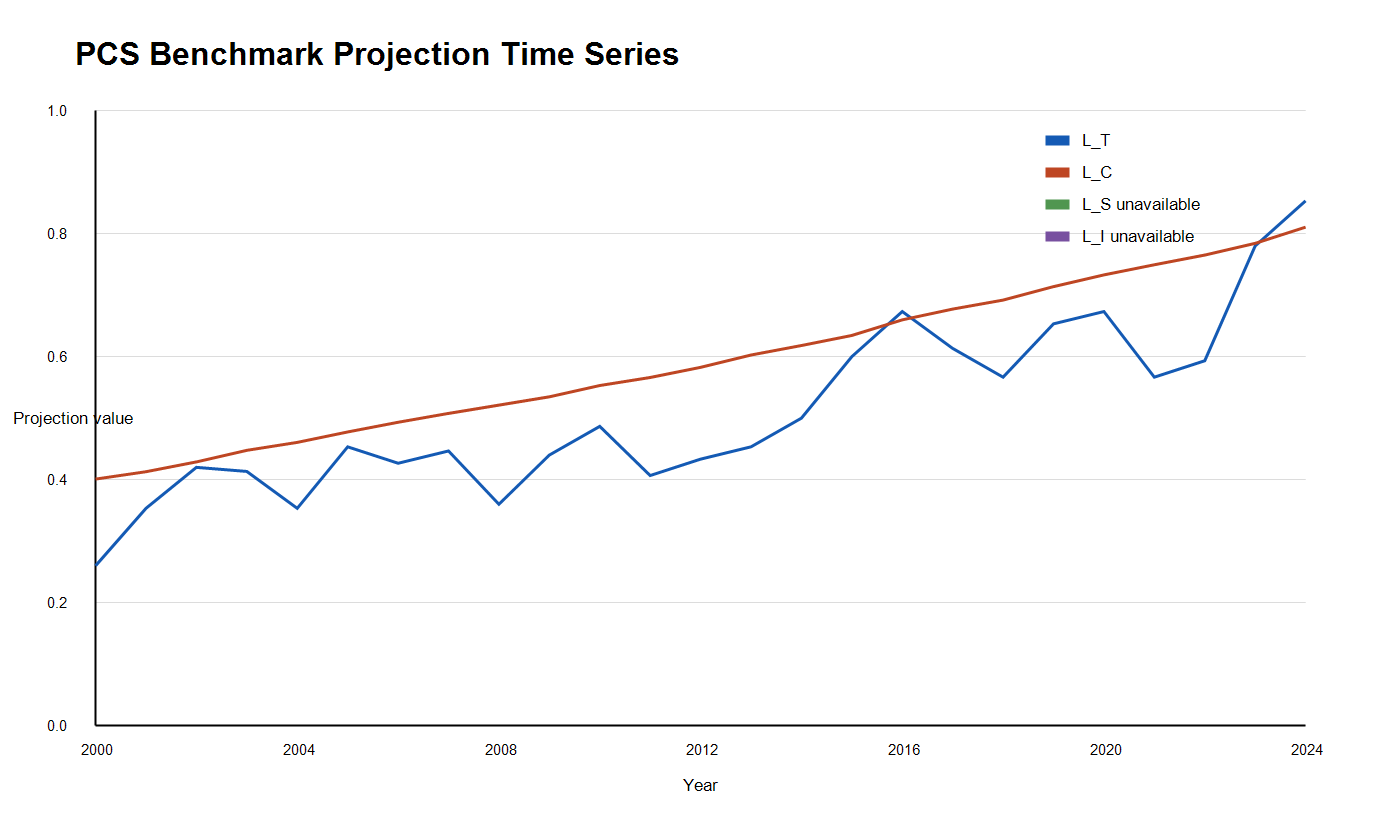
\includegraphics[width=\columnwidth]{figures/fig11_projection_timeseries.png}
\caption{Projection time series for the PCS benchmark demonstration.}
\label{fig:projection_timeseries}
\end{figure}

The thermal projection \(L_T\) covers 2000--2024, ranges from 0.260000 to 0.853333, and has mean 0.511200. The chemical projection \(L_C\) covers the same interval, ranges from 0.400910 to 0.810551, and has mean 0.593097. The structural and informational projections are unavailable and remain `NaN`.

Figure~\ref{fig:demo_statistics} summarizes the demo-state statistics. The demo state \(S_{\mathrm{demo}}\) ranges from 0.330455 to 0.831942, with mean 0.552148. The total change from 2000 to 2024 is 0.501487, and the fitted annual trend is approximately 0.017054 per year.

\begin{figure}[tb]
\centering
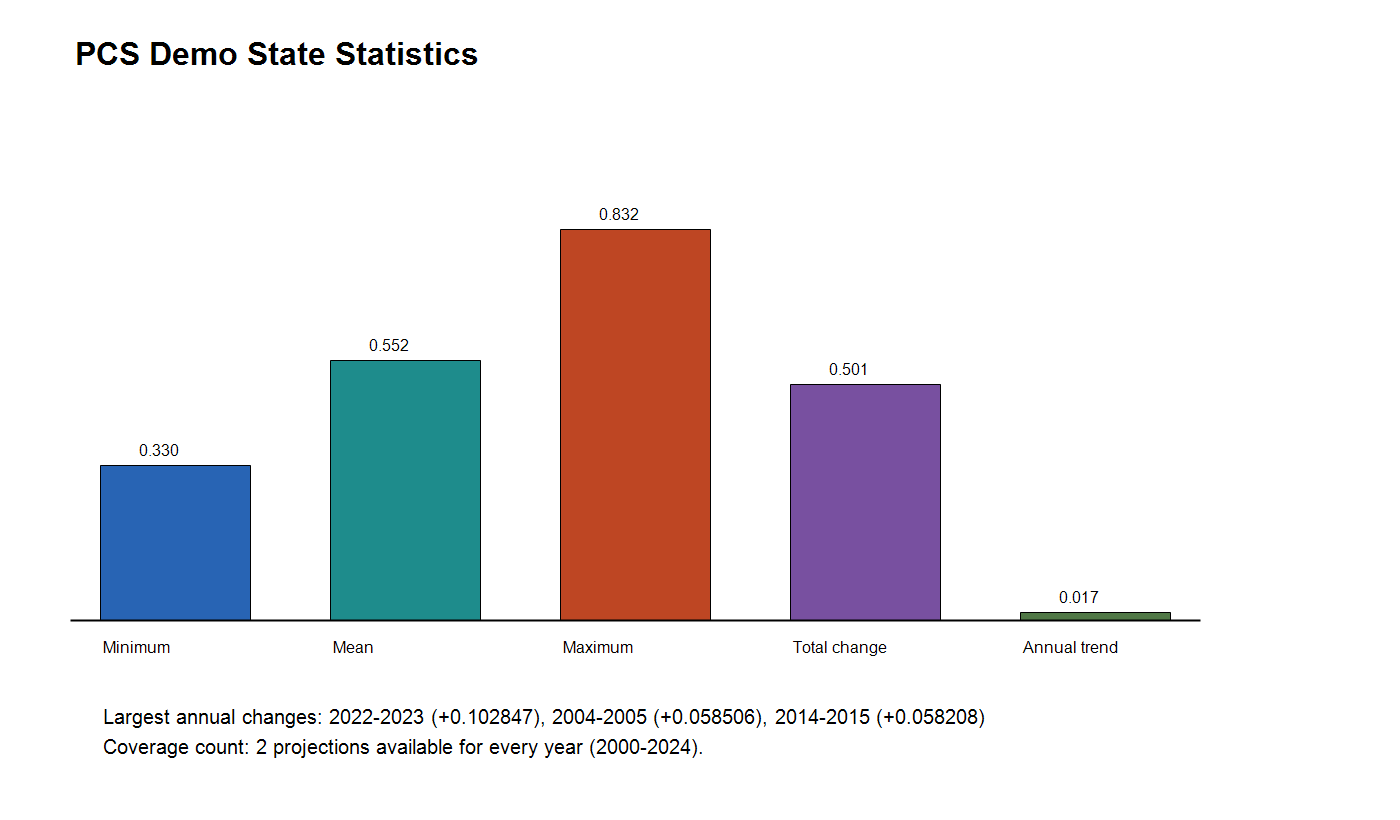
\includegraphics[width=\columnwidth]{figures/fig12_demo_statistics.png}
\caption{Summary statistics for the PCS demo state.}
\label{fig:demo_statistics}
\end{figure}

Table~\ref{tab:demo_summary} summarizes the demo-state statistics. The largest annual increase occurs in 2022--2023, with a change of 0.102847. This change is consistent with the large increase in \(L_T\) over the same interval while \(L_C\) continues its smooth increase.
\begin{table}[tb]
\caption{\label{tab:demo_summary}Summary statistics for \(S_{\mathrm{demo}}\).}
\footnotesize
\begin{ruledtabular}
\begin{tabular}{ll}
Statistic & Value \\
Minimum & 0.330455 \\
Maximum & 0.831942 \\
Mean & 0.552148 \\
Total change, 2000--2024 & 0.501487 \\
Linear annual trend & 0.017054 yr\(^{-1}\) \\
Largest annual change & 2022--2023: 0.102847 \\
Coverage count & 2 in all years \\
\end{tabular}
\end{ruledtabular}
\end{table}


\subsection{9.6 Limitations}

This benchmark is an operational demonstration, not a validation study. No predictive claim is made. The benchmark does not test forecasting skill, causal structure, or model performance against independent targets. It only verifies that the projection and aggregation procedure behaves consistently for the available observations.

The demonstration is incomplete because \(L_S\) and \(L_I\) are unavailable. As a result, \(S_{\mathrm{demo}}\) is computed from two available projections rather than the intended four-projection benchmark state. The normalization constants are demonstration choices specified in the PCS Projection Standard v1.0 and should not be interpreted as universal thresholds.

\subsection{9.7 Reproducibility}

The benchmark data are stored in `PCS_DATA/processed/demo_annual_dataset.csv` and `PCS_DATA/normalized/demo_projection_dataset.csv`. The raw-source excerpts and acquisition notes are stored under `PCS_DATA/raw/`, and the dataset manifest is stored under `PCS_DATA/metadata/`.

The benchmark preserves missing values as `NaN`, does not interpolate unavailable datasets, and records `coverage_count` for each year. Future extensions should add authenticated NASA global mean sea-level data and processed MODIS MOD13C2 annual global NDVI aggregates, after which the demo state can be recomputed with all four projections.
